% Generated support snippets from ScytaleDroid cutoff-window and static audit outputs.
% These snippets are optional support material; keep manuscript claims aligned with the 14-day cutoff-window model.

\begin{table}[t]
\caption{Cutoff-window evidence summary.}
\label{tab:cutoff-window-summary-generated}
\centering
\begin{tabular}{p{0.58\linewidth}p{0.22\linewidth}}
\toprule
Metric & Value \\
\midrule
Apps with recent build-backed evidence & 15/15 \\
Apps with selected evidence in 14-day window & 15/15 \\
True evidence holes & 0 \\
PCAP-backed dynamic runs & 123 \\
Strict idle captures & 44 \\
Quiescent foreground captures & 23 \\
Interactive captures & 56 \\
\bottomrule
\end{tabular}
\end{table}

\begin{table*}[t]
\caption{Selected build-backed evidence bundle by application. Runtime classes are strict idle/quiescent foreground/interactive.}
\label{tab:app-evidence-generated}
\centering
\scriptsize
\begin{tabular}{llrccr}
\toprule
App & Version & Last capture & I/Q/Int & PCAPs & Static risk \\
\midrule
BBC News & 2026.5.0 & Jul. 7 & 4/0/6 & 10 & 0.72 \\
CNN & 26.13.0 & Jul. 9 & 4/1/7 & 12 & 0.12 \\
LinkedIn & 4.1.1218 & Jul. 9 & 3/1/4 & 8 & 4.08 \\
Telegram & 12.8.3 & Jul. 9 & 3/0/4 & 7 & 6.59 \\
Signal & 8.18.2 & Jul. 9 & 3/0/4 & 7 & 5.52 \\
Pinterest & 14.26.0 & Jul. 9 & 5/0/2 & 7 & 2.84 \\
Snapchat & 14.14.0.43 & Jul. 9 & 1/2/2 & 5 & 6.04 \\
Facebook & 567.1.0.52.74 & Jul. 6 & 3/1/4 & 8 & 6.00 \\
Messenger & 567.1.0.53.87 & Jul. 7 & 4/0/5 & 9 & 5.88 \\
Guardian & 6.226.23011 & Jul. 6 & 3/2/4 & 9 & 0.74 \\
Instagram & 436.0.0.41.73 & Jul. 7 & 2/4/1 & 7 & 5.48 \\
Reddit & 2026.26.0 & Jul. 9 & 2/3/1 & 6 & 3.16 \\
X & 12.5.0-release.0 & Jul. 6 & 3/1/4 & 8 & 4.48 \\
WhatsApp & 2.26.25.80 & Jul. 6 & 4/0/5 & 9 & 7.55 \\
TikTok & 45.7.3 & Jul. 6 & 0/8/3 & 11 & 4.40 \\
\bottomrule
\end{tabular}
\end{table*}

\begin{figure*}[t]
\centering
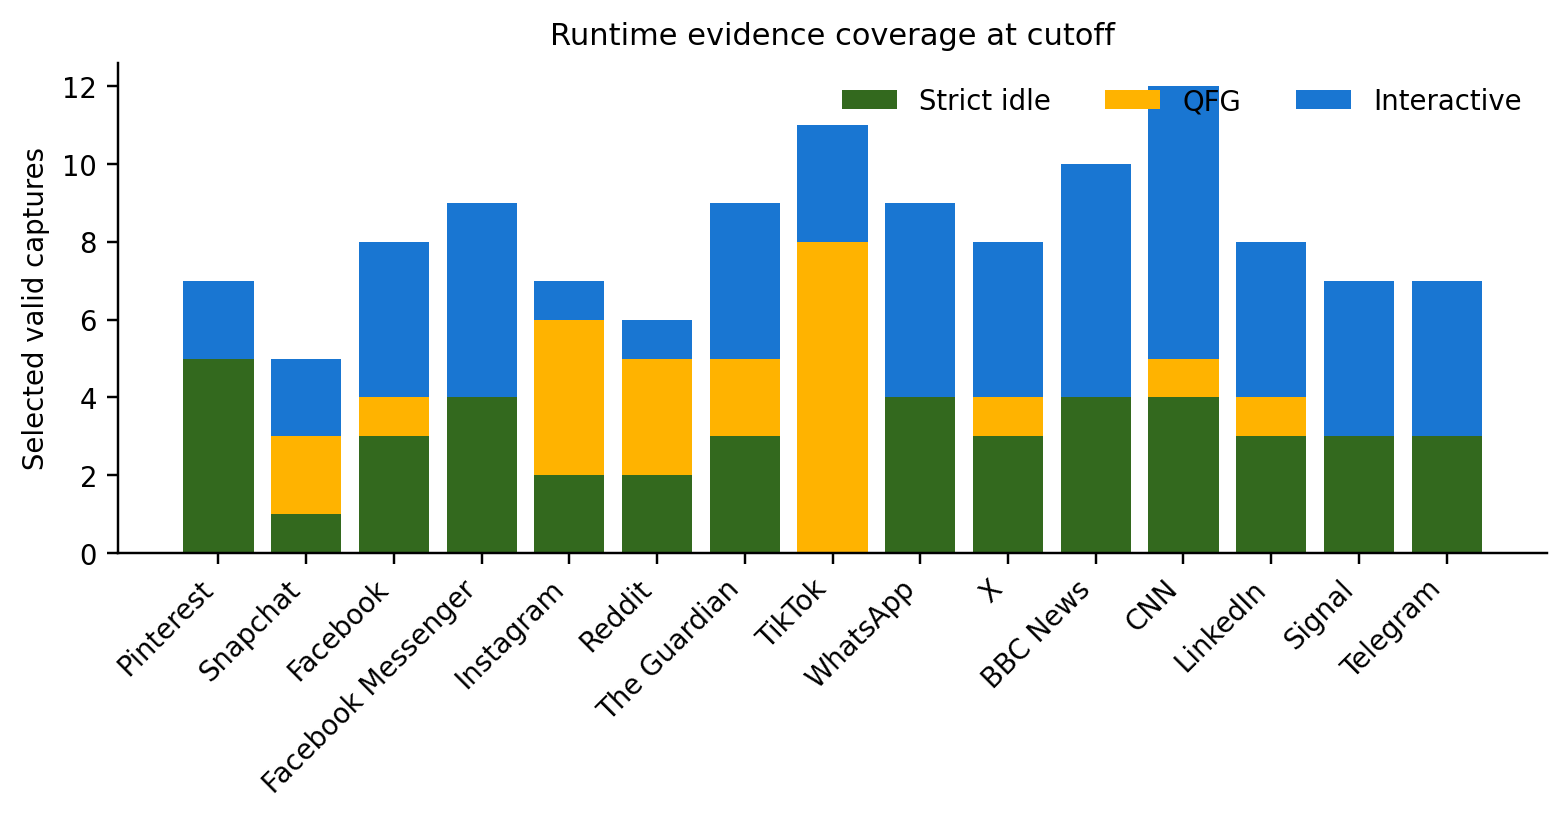
\includegraphics[width=0.95\linewidth]{assets/figures/runtime_coverage_by_app.png}
\caption{Runtime evidence coverage by app at cutoff. Strict idle, quiescent foreground, and interactive captures are kept separate.}
\label{fig:runtime-coverage-generated}
\end{figure*}

\begin{figure}[t]
\centering
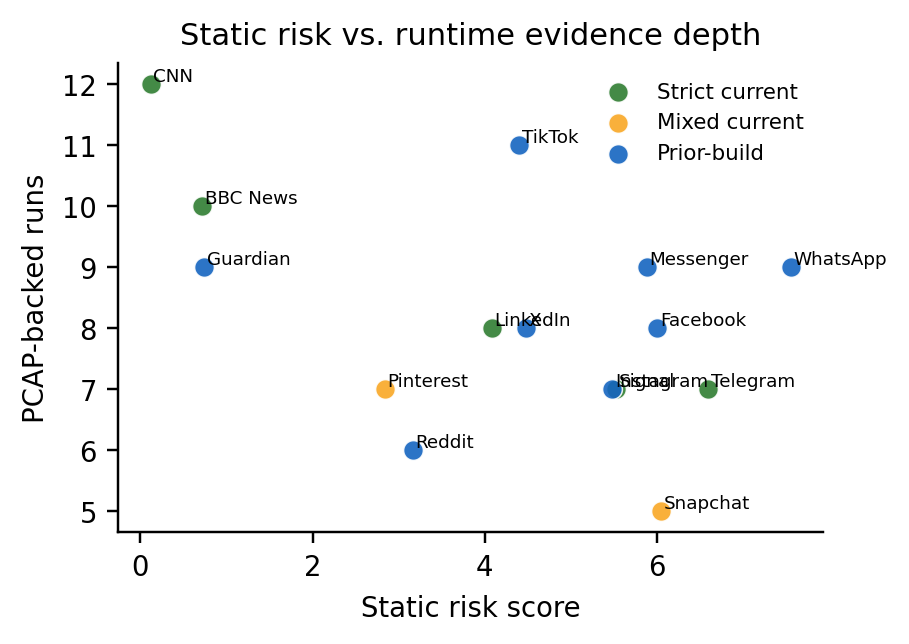
\includegraphics[width=0.98\linewidth]{assets/figures/static_risk_vs_pcap.png}
\caption{Static risk score versus PCAP-backed runtime evidence count for selected app bundles.}
\label{fig:static-runtime-scatter-generated}
\end{figure}
